%%%%%%%%%%%%%%%%%%%%%%%%%%%%%%%%%%%%%%%%%%%%%%%%%%%%%%%%%%%%%%%%%%%%%%%%%%%%%%%
%
% Tommy P. Keane
% Master of Science Thesis
% Department of Electrical and Microelectronic Engineering
% Rochester Institute of Technology
%
% April 2011
%
%
%
% Funded By: Lenel Systems Inc., A UTC Fire & Security Corporation
%
% Algorithm Intellectual Property Owned By: Lenel Systems Inc.
%
%
% http://www.tommypkeane.com
%
%%%%%%%%%%%%%%%%%%%%%%%%%%%%%%%%%%%%%%%%%%%%%%%%%%%%%%%%%%%%%%%%%%%%%%%%%%%%%%%

%%%%%%%%%%%%%%%%%%%%%%%%%%%%%%%%%%%%%%%%%%%%%%%%%%%%%%%%%%%%%%%%%%%%%%%%%%%%%%%
%
% CHAPTER 4
%
% SECTION 3: Complex Views
%
%%%%%%%%%%%%%%%%%%%%%%%%%%%%%%%%%%%%%%%%%%%%%%%%%%%%%%%%%%%%%%%%%%%%%%%%%%%%%%%


%%%%%%%%%%%%%%%%%%%%%%%%%%%%%%%%%%%%%%%%%%%%%%%%%%%%%%%%%%%%%%%%%%%%%%%%%%%%%%%
% BEGIN DOCUMENT

This final set of results are all realistic scenarios for surveillance, most of which come from real, stationary security cameras. The real surveillance image sets are much poorer in quality as they are susceptible to all the previously discussed weather and illumination artifacts. The cameras are usually not as good quality as a commercial personal use camera (from which all the previous images were taken, as well as the sets in Figures \ref{ArtGallery1Images} and \ref{ArtGallery2Images}). So these results show the strength of the algorithm not only for its use of a simple affine search in the face of occlusion and parallax disparities, but also in the face of real noise, real illumination variations, and truly unknown and uncontrolled camera parameters. As with all the results a very simple stitching seam (vertically halfway through the overlap region) was chosen and it is visible in all of the following results as none of these scenes are mathematically relatable by only an affine homography. However, all the results present an accurate estimate for the overlap region with no added complexity from the previous scenarios. These are all based on simple and fast calculations, that still have room for optimization to real time operation, and while ``ghosting'' and ``jumps'' are very visible, the views present a convincing panorama of the scene that is easily understood by a viewer. Especially given the color variations and depth discrepancies between the views, it can be a challenge (when unfamiliar with the scenes) to understand the true relationship between the views. These views, as all the previous ones, are generally of size $480 \times 640$ (row by column) and with all the implementation features mentioned in the previous chapter, they can be run through the entire algorithm (including being read in, stitched, and written out to file) in about 10 minutes for a modest search space in the MATLAB\textsuperscript{\textregistered} implementation. The OpenCV implementation was not completed for the entire algorithm, but the core components (transformation search, registration, and blending) were implemented and ran in less than a minute with very modest hardware specifications in both methods (Intel\textsuperscript{\textregistered} Core 2 Duo with 2GB RAM). There is room for improvement, but this is clearly a robust and useful metric for registration and has been presented as a novel solution to a very complex problem as these scenes have all the problems that are typically avoided by most registration algorithms and are often only tackled one at a time, rarely does it occur that an algorithm attempts to overcome so many issues simultaneously with a combined effort and gestalt view of the problems and scenarios. That is the strength and core of this algorithm, that all the various problems come down to producing real, singular images; images of interest don't typically have one or two problems, they have them all, and so in designing an algorithm to overcome a problem it should take into consideration where and when that problem occurs, and often that will be alongside many other problems which cannot be ignored.

Manually registered views are not presented for comparison as it would be pointless to attempt to manually register these views with a clearly irrelevant affine homography. To show the views registered manually and accurately would also be pointless as it does not enhance an understanding of where the errors occur as they are all very visible, and the correct views would be distorted in a 3-D space, and thus irrelevant to compare to results restricted to the 2-D image planes.

\newpage

% ART GALLERY 001
\begin{figure}
\centering
\subfigure{ 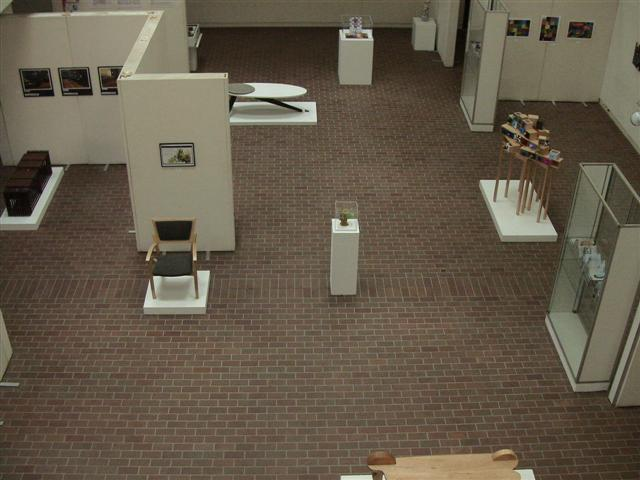
\includegraphics[width=.45\textwidth]{AGS1L001} \label{ArtGallery1L} }
\subfigure{ 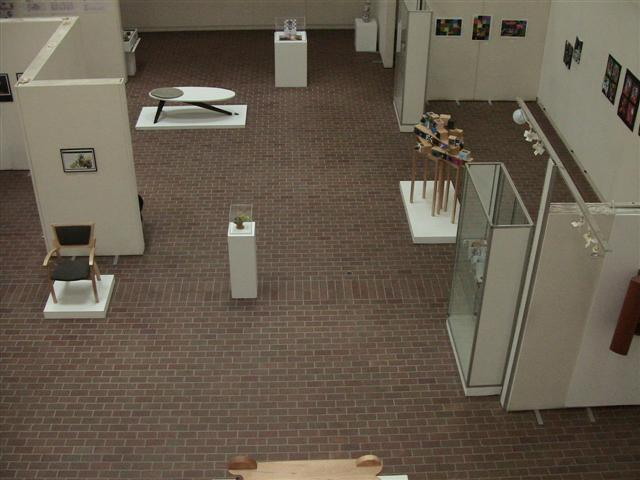
\includegraphics[width=.45\textwidth]{AGS1R001} \label{ArtGallery1R} }
\caption{Art Gallery Scene 01 (a) Left View, (b) Right View}
\label{ArtGallery1Images}
\end{figure}

\begin{figure}
\centering
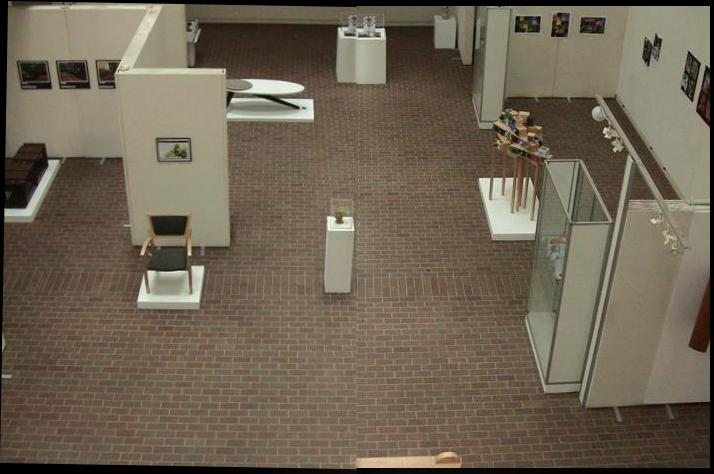
\includegraphics[width=1\textwidth]{AGS1SP001001}
\caption{Art Gallery 01 Views Blended}
\label{ArtGallery1Stitched}
\end{figure}




% ART GALLERY 002
\begin{figure}
\centering
\subfigure{ 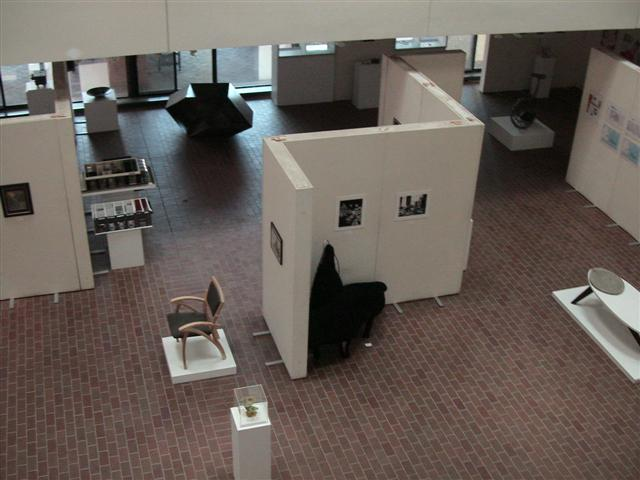
\includegraphics[width=.45\textwidth]{AGS2L001} \label{ArtGallery2L} }
\subfigure{ 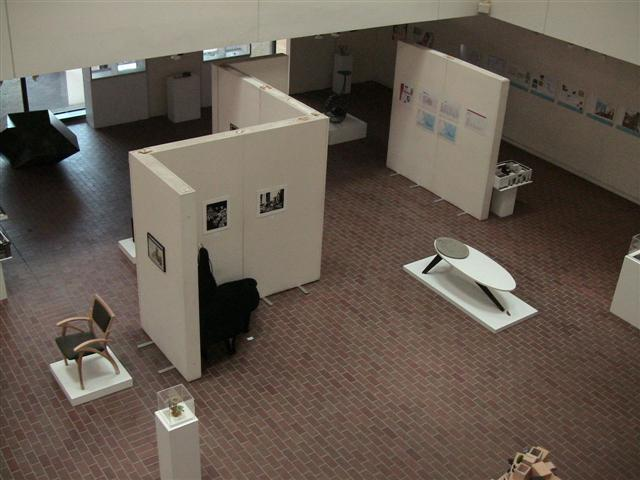
\includegraphics[width=.45\textwidth]{AGS2R001} \label{ArtGallery2R} }
\caption{Art Gallery Scene 02 (a) Left View, (b) Right View}
\label{ArtGallery2Images}
\end{figure}

\begin{figure}
\label{ArtGallery2Stitched}
\centering
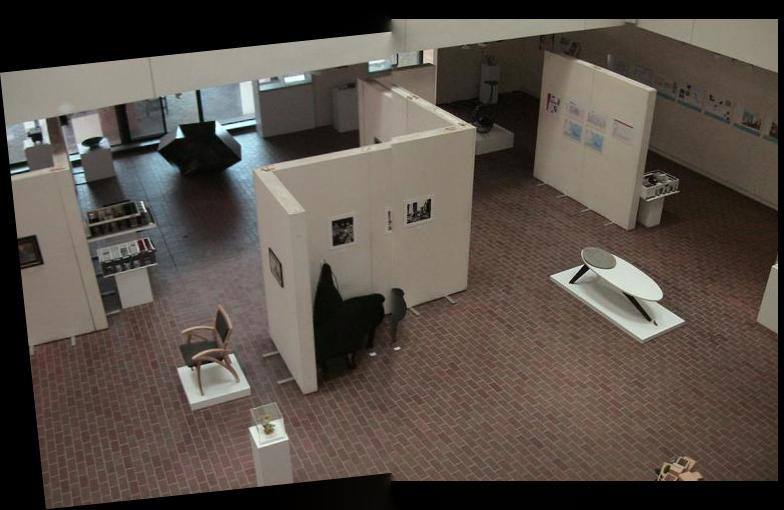
\includegraphics[width=1\textwidth]{AGS2SP001001}
\caption{Art Gallery 02 Views Blended}
\end{figure}



% LENEL 005
\begin{figure}
\centering
\subfigure{ 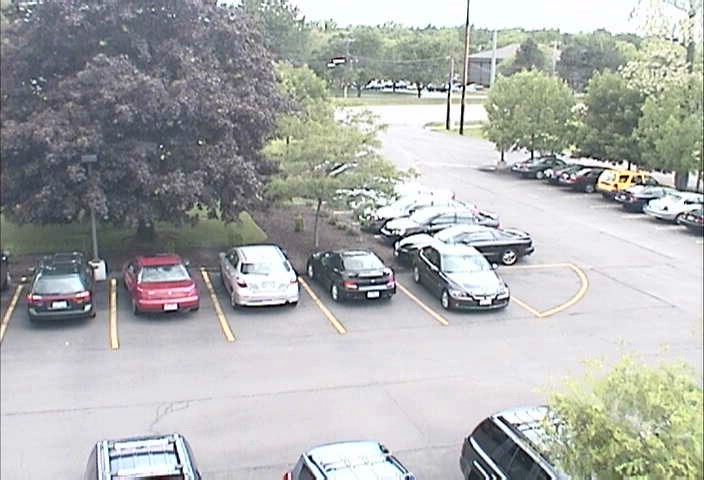
\includegraphics[width=.45\textwidth]{Lenel005L001} \label{Lenel5L} }
\subfigure{ 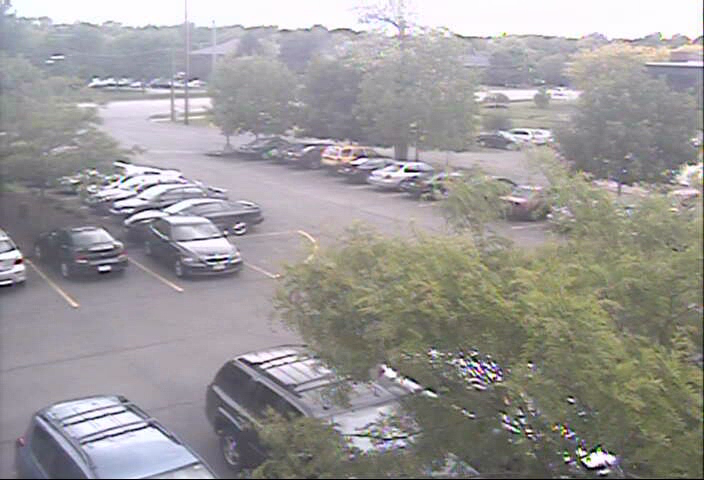
\includegraphics[width=.45\textwidth]{Lenel005R001} \label{Lenel5R} }
\caption{Lenel Front Lot Scene (a) Left View, (b) Right View}
\label{Lenel5Images}
\end{figure}

\begin{figure}
\centering
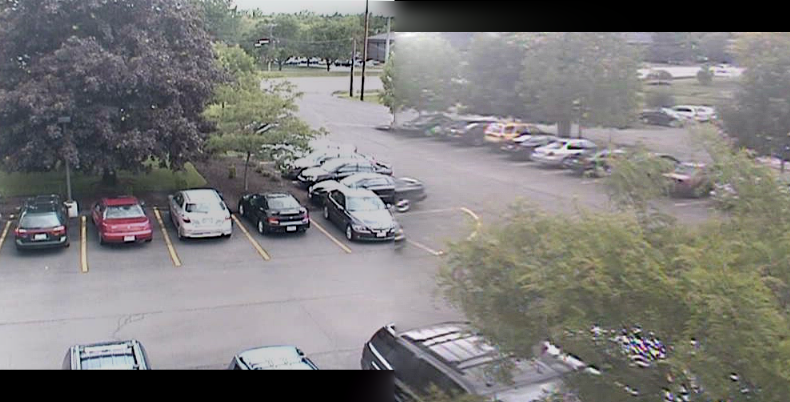
\includegraphics[width=1\textwidth]{Lenel005SP001001}
\caption{Lenel Front Lot Views Blended}
\label{Lenel5Stitched}
\end{figure}



% LENEL 010
\begin{figure}
\centering
\subfigure{ 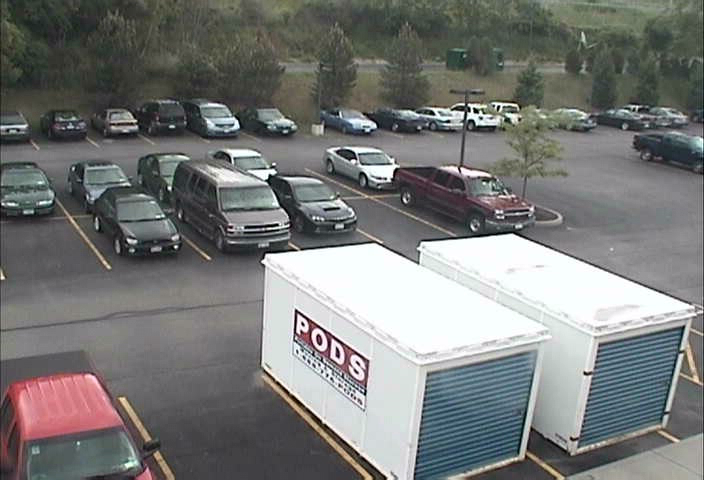
\includegraphics[width=.45\textwidth]{Lenel010L004} \label{Lenel10L} }
\subfigure{ 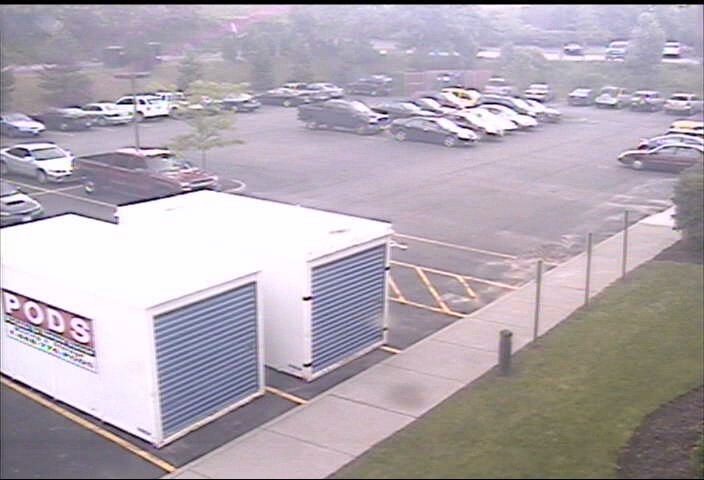
\includegraphics[width=.45\textwidth]{Lenel010R004} \label{Lenel10R} }
\caption{Lenel Back Lot Scene (a) Left View, (b) Right View}
\label{Lenel10Images}
\end{figure}

\begin{figure}
\centering
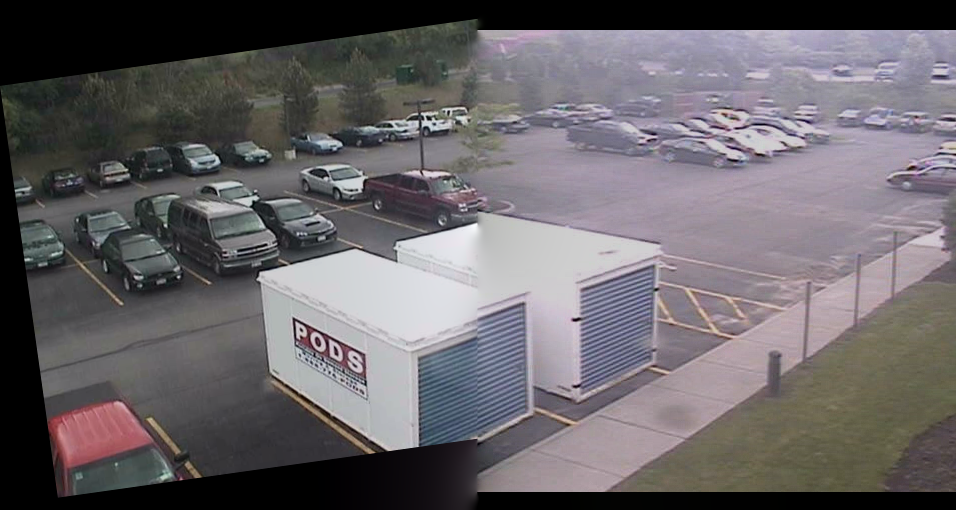
\includegraphics[width=1\textwidth]{Lenel010SP001}
\caption{Lenel Back Lot Views Blended}
\label{Lenel10Stitched}
\end{figure}


%%%%%%%%%%%%%%%%%%%%%%%%%%%%%%%%%%%%%%%%%%%%%%%%%%%%%%%%%%%%%%%%%%%%%%%%%%%%%%%
% END OF DOCUMENT

